\section{Modello del sistema}
Il sistema consiste in un pendolo rigido, libero di ruotare e vincolato a muoversi lungo una rotaia rettilinea tramite un carrello.
L'unico controllo che ho sul sistema è
una forza applicata sul carrello lungo la direzione della rotaia,
così come è mostrato in \autoref{fig:pic}.
Io sono interessato
ad applicare questo studio nel mondo reale, quindi devo tenere
in considerazione che la forza è generata da un motore in risposta
a un segnale di input; in particolare, uso un motore elettrico a corrente continua
a spazzole. Visto che il motore è un sistema dinamico in sé,
è conveniente modellarlo separatamente rispetto al sistema
carrello-pendolo.
In \autoref{fig:pic-real} è
mostrato uno schema del sistema reale.

\begin{figure}[h]
    \centering
    \begin{subfigure}[b]{0.48\textwidth}
        \centering
        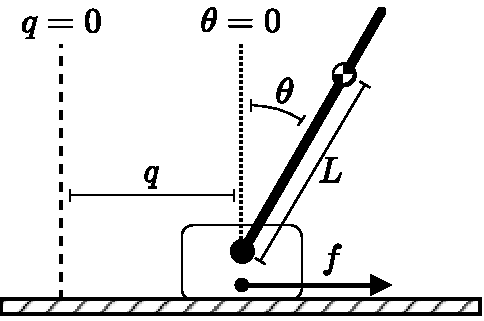
\includegraphics[width=\textwidth]{assets/pic}
        \caption{Schema ideale del sistema. La forza di controllo esterna
        agisce direttamente sul carrello, nella direzione dello scorrimento.}
        \label{fig:pic}
    \end{subfigure}
    \hfill
    \begin{subfigure}[b]{0.48\textwidth}
        \centering
        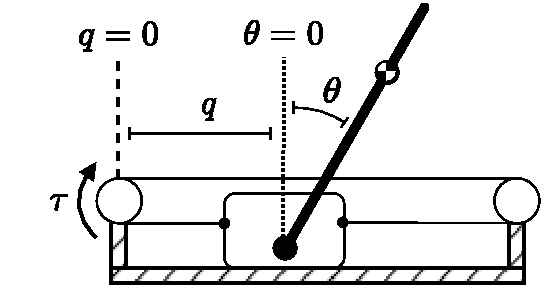
\includegraphics[width=\textwidth]{assets/pic-real}
        \caption{Schema reale del sistema. La forza di controllo viene
        generata da un motore e trasferita al carrello con una cinghia.}
        \label{fig:pic-real}
    \end{subfigure}
    \caption[Schema del sistema ideale e reale]{Schema del sistema ideale e reale. Nelle figure sono mostrate le variabili
    utilizzate.}
\end{figure}



\subsection{Pendolo e carrello}
Riporto i parametri e le variabili d'interesse per il sistema in 
\autoref{tab:parametri} e ricavo le equazioni del moto
usando l'approccio Lagrangiano.
Energia cinetica e potenziale sono
\begin{align*}
        T &= \frac 1 2 M  \dot q^2 + \frac 1 2 m v_{cm}^2 + \frac 1 2 (I - lm^2)\dot \theta^2, \\
        V &= mgl \cos\theta
\end{align*}
dove $v_{cm}$ è la velocità del centro di massa del pendolo, data da
\begin{equation*}
    v^2_{cm} = (\dot x + l \dot \theta \cos \theta)^2 + (l \dot \theta \sin \theta)^2.
\end{equation*}

Scrivo la Lagrangiana del sistema
\begin{equation*}
    \mathcal L = T - V
\end{equation*}
e imposto le equazioni di Eulero-Lagrange:

\begin{equation}
        \left\{
        \begin{aligned}
            \totald t \partiald{\dot q} {\mathcal L} - \partiald q {\mathcal L} &= f \\
            \totald t \partiald{\dot \theta} {\mathcal L}  - \partiald \theta {\mathcal L} &= 0
        \end{aligned}
        \right.
        \label{eq:eulero-lagrange-pendolo}
\end{equation}
in cui trascuro gli attriti tra carrello e rotaia e tra
pendolo e perno.
Dal sistema~\eqref{eq:eulero-lagrange-pendolo} ricavo le equazioni del moto:
\begin{equation}
        \left\{
        \begin{aligned}
            \ddot x &= \frac {-lm \ddot \theta \cos \theta + lm \dot \theta^2 \sin \theta + f} {m + M} \\
            \ddot \theta &= \frac {lm (g\sin \theta - \cos \theta) }{I} \ddot x
        \end{aligned}
    \right.
    _.
    \label{eq:moto-sistema}
\end{equation}
Concludo studiando i punti di equilibrio del sistema.
L'unica variabile che compare nel potenziale è $\theta$; impongo
\begin{equation*}
    \left. \frac \partial {\partial \theta}\right |_{V=V_{eq}} V =  0
\end{equation*}
da cui
\begin{equation*}
     V_{eq} = \{0, \pi\}.
\end{equation*}
La stabilità è data da considerazioni fisiche
\begin{align*}
    \theta &= 0  \text{ è instabile}, \\
    \theta &= \pi  \text{ è stabile}.
\end{align*}

\bgroup
\renewcommand{\tabularxcolumn}[1]{>{\arraybackslash}m{#1}}
\renewcommand\arraystretch{1.5}
\begin{table}[h]
    \centering
    \begin{tabularx}{\textwidth}{| gc | X |}
        \noalign{\hrule height 2pt}

        \rowcolor{Black}%

        \multicolumn{1}{=c}{\rowstyle{\bfseries\sffamily \color{White}} Parametro/Variabile} & \multicolumn{1}{+c}{ Descrizione} \\
        \hline
        $g$ & Accelerazione di gravità. \\
        \hline
        $M$ & Massa del carrello. \\
        \hline
        $m$ & Massa del pendolo. \\
        \hline
        $l$ & Distanza tra il centro di massa del pendolo e il punto di rotazione. \\
        \hline
        $I$ & Momento d'inerzia del pendolo calcolato rispetto al punto di rotazione. \\
        \hline
        $q$ & Posizione del carrello rispetto all'origine. \\
        \hline
        $\theta \in ]-\pi, +\pi]$ & Angolo del pendolo rispetto alla verticale. \\
        \hline
        $f$ & Forza agente sul carrello. \\
        \noalign{\hrule height 2pt}
    \end{tabularx}
    \caption{Descrizione di parametri e variabili del sistema carrello-pendolo.}
    \label{tab:parametri}
\end{table}
\egroup

\subsection{Motore}
\label{subsec:modello-motore}
Lavoro con un motore \textsc{DC} a spazzole.
Riporto i parametri e le variabili d'interesse per il motore in \autoref{tab:parametri-motore}.
Si può ricavare~\cite{Zaccarian} che valgono le equazioni
\begin{subequations}
    \begin{empheq}[left=\empheqlbrace,right=_.]{align}
            u &= L_a \dot J + R_a J + K_e \omega \label{eq:motore-1} \\
            \tau &= K_m J \label{eq:motore-2}
    \end{empheq}
\end{subequations}

Voglio ricavare la forza esercitata dal motore in funzione di $u$.
Dalla~\eqref{eq:motore-2} ricavo
\begin{equation}
        \dot J = \totald t \left( \frac \tau {K_m}\right) = \frac{\dot \tau}{K_m}
        \label{eq:jdot}
\end{equation}
e inserendo la~\eqref{eq:jdot} nella~\eqref{eq:motore-1} ottengo
\begin{equation}
        u = \frac {L_a} {K_m} \dot\tau + \frac{R_a}{K_m}  \tau + K_e \omega.
        \label{eq:u-motore}
\end{equation}
Considero la~\eqref{eq:u-motore} in regime stazionario\footnote{
Spiegherò il motivo di questa scelta nel paragrafo~\ref{sec:sistema-reale}.
In genere sono autorizzato a fare questa semplificazione quando la scala dei tempi
elettrica del motore, data da $\sfrac {R_a}{L_a}$, è più grande del tempo medio
che passa tra un input $u$ e il successivo.
} ($\dot \tau = 0$).
Dato che $\tau \propto f$ e $\omega \propto \dot q$ ottengo
\begin{equation}
    u = A f + B \dot q.
    \label{eq:caratteristica-motore}
\end{equation}
Il segnale di controllo del motore
dipende quindi solo da due parametri $A$ e $B$ determinabili sperimentalmente.

\bgroup
\renewcommand{\tabularxcolumn}[1]{>{\arraybackslash}m{#1}}
\renewcommand\arraystretch{1.5}
\begin{table}[t]
    \centering
    \begin{tabularx}{\textwidth}{| gc | X |}
        \noalign{\hrule height 2pt}

        \rowcolor{Black}%
        \multicolumn{1}{=c}{\rowstyle{\bfseries\sffamily \color{White}} Parametro/Variabile} & \multicolumn{1}{+c}{ Descrizione} \\
        \hline
        $L_a$ & Induttanza delle armature. \\
        \hline
        $R_a$ & Resistenza delle armature. \\
        \hline
        $K_e$ & Costante elettrica del motore. \\
        \hline
        $K_m$ & Costante meccanica del motore. \\
        \hline
        $u$ & Differenza di potenziale tra le armature. \\
        \hline
        $J$ & Corrente che scorre nelle armature. \\
        \hline
        $\tau$ & Coppia esercitata dal motore. \\
        \hline
        $\omega$ & Velocità angolare del motore. \\
        \hline
        $f$ & Forza agente sul carrello. \\
        \hline
        $\dot q$ & Velocità del carrello. \\
        \noalign{\hrule height 2pt}
    \end{tabularx}
    \caption{Descrizione di parametri e variabili del motore.}
    \label{tab:parametri-motore}
\end{table}
\egroup